\section{Introduction}
Several attempts have been made to improve upon the lossy image compression offered by \textsc{jpeg} \cite{ginesu2012objective} \cite{toderici2016full}.
Despite these efforts, \textsc{jpeg} continues to be the standard image file format on the web.
Because of the status of \textsc{jpeg} as the default standard and its wide adoption, it seems unlikely that the new formats will get any traction.
We propose an image compression technique to improve the visual quality of standard \textsc{jpeg} by using a higher bitrate to encode image regions flagged by our model as containing an object of interest and lowering the bitrate elsewhere in the image.
The compressed output of our method can be decoded by standard \textsc{jpeg} implementations.

The \textsc{jpeg} algorithm uses a scaling factor $Q$ in order to scale the quantization matrix to achieve a variety of compression ratios.
However, this ratio is an image level property and all the $8 \times 8$ blocks of a given image are compressed using the same scaling factor.
Natural images are heterogeneous with respect to frequency, and contain both regions of primarily low frequencies and of primarily high frequencies.
While low frequency regions are more tolerant of higher compression ratios, high frequency regions are not \cite{chandra1999jpegcompressionme}.
Therefore, variable quantization in \textsc{jpeg} would aim to provide optimum perceptual quality across the image by compressing different blocks at different ratios.
Previous approaches to use variable quantization have employed DCT analysis on each block to determine the frequency components \cite{konstantinides1998method} as well as classification of each block according to a pre-determined look-up table \cite{memon2000method}.
Soon et al \cite{tan1996classified} proposed classifying blocks as textures, edges or flat regions, and adjusting the quantization matrix for each block accordingly.
Adaptive Quantization techniques have also been applied to video coding \cite{xiang2014adaptive}.

These methods are limited in their ability to improve the perceptual quality of an image because frequency analysis and image metrics do not correlate with human perception \cite{klein1992relevance}.
Therefore, we propose variable quantization of \textsc{jpeg} in which the choice of scaling factor is informed by semantic knowledge of the image.
Human vision naturally focuses on familiar semantic objects, and is particularly sensitive to distortions of these objects as compared to distortions of background details.
Our goal is to develop a technique which improves the visual quality of an image by improving the signal to noise ratio within these semantic objects while keeping the overall visual quality close to that of standard \textsc{jpeg}. 
Measuring visual quality is an ongoing research area and there is no consensus among researchers on the proper metric. 
We evaluate our model on a variety of metrics, \texttt{SSIM}\cite{ssim}, \texttt{MS-SSIM}\cite{msssim}, \texttt{VIFP}\cite{vifp}, \texttt{PSNR-HVS}\cite{psnrhvs} and \texttt{PSNR-HVSM}\cite{psnrhvsm}; these robust metrics have been shown to correlate better with subjective quality measurement than pixel-level metrics such as \texttt{MSE} or \texttt{PSNR} \cite{psnrhvsm}.
Yuri et al \cite{kerofsky2015perceptual} showed that \texttt{PSNR} as an image comparison metric has severe limitations.

Convolutional Neural Networks (\textsc{cnn}s) have been successfully applied to a variety of computer vision tasks \cite{he2015deep} \cite{krizhevsky2012imagenet}.
Their feature extraction and transfer learning capabilities are now well known\cite{zeiler2014visualizing} .
\textsc{cnn}s, well known for their ability to classify images by their most prominent object, and have also been used to draw a bounding box around that object \cite{girshick2014rich}.
This method is capable of providing a binary map for the presence of the most salient object. Some success has been obtained in predicting the visual saliency map of a given image \cite{jiang2015salicon} \cite{kummerer2014deep}.

We propose a deep convolution network designed to locate several semantic objects within a single image.
Our model differs from traditional object detection models like \cite{dai2016r} \cite{girshick2014rich} as these models are restricted to detecting a single salient object in an image, typically an instance of a pre-computed class for that image.
Previous work has shown that semantic object detection has a variety of advantages over saliency maps \cite{mnih2014recurrent} \cite{zund2013content}. Semantic detection models recognize discrete objects and are thus able to generate maps that are more coherent for human perception.
% done: consider comparing ground-truth heatmap with model's heatmap -- NOT enough SPACE
Visual saliency models are based on human eye fixations, and thus produce results which do not capture object boundaries.
This is particularly evident in the results obtained by Stella et al \cite{stella2009image}, in which image compression is guided by a multi-scale saliency map, and the obtained images show blurred edges and soft focus.
Our proposed model captures the structure of the depicted scene and thus maintains the integrity of semantic objects, unlike results produced using human eye fixations \cite{liu2015predicting}.


Our proposed model produces a single class-invariant feature map by learning separate feature maps for each of a set of object classes and then summing over the top features.
Our model trades lower confidence of bounding edges for the ability to find all salient regions of an image in a single pass, as opposed to standard object-detection \textsc{cnn}s, which require multiple passes over the image to identify and locate all the objects.
In comparison to grid-based features as described by Yuri et al \cite{reznik2013coding} our features are scale- and transformation-invariant, which allows application of the model to a wider class of images.

We employ a Convolutional Neural Network (\textsc{cnn}) tailored to the specific task of semantic image understanding to achieve higher visual quality in lossy image compression.
We focus on the \textsc{jpeg} standard, which remains the dominant image representation on the internet and in consumer electronics. 
Several attempts have been made to improve upon its lossy image compression, for example WebP \cite{ginesu2012objective} and Residual-GRU \cite{toderici2016full}, but many of these require custom decoders and are not sufficiently content-aware.

We improve the visual quality of standard \textsc{jpeg} by using a higher bit rate to encode image regions flagged by our model as containing content of interest and lowering the bit rate elsewhere in the image. 
With our enhanced \textsc{jpeg} encoder, the quantization of each region is informed by knowledge of the image content.
Human vision naturally focuses on familiar objects, and is particularly sensitive to distortions of these objects as compared to distortions of background details \cite{jiang2015salicon}.
By improving the signal-to-noise ratio within multiple regions of interest, we improve visual quality of those regions, while preserving overall \texttt{PSNR} and compression ratio.
A second encoding pass produces a final \textsc{jpeg} encoding that may be decoded with any standard off-the-shelf \textsc{jpeg} decoder.
Measuring visual quality is an ongoing area of research and there is no consensus among researchers on the proper metric.
Yuri et al \cite{kerofsky2015perceptual} showed that \texttt{PSNR} has severe limitations as an image comparison metric.
Richter et al \cite{richter2009ms}\cite{richter2011ssim} addressed structural similarity (\texttt{SSIM}\cite{ssim} and \texttt{MS-SSIM}\cite{msssim}) for \textsc{jpeg} and \textsc{jpeg} 2000.
We evaluate on these metrics, as well as \texttt{VIFP}\cite{vifp},  \texttt{PSNR-HVS}\cite{psnrhvs} and \texttt{PSNR-HVSM}\cite{psnrhvsm}, which have been shown to correlate with subjective visual quality.  Figure~\ref{fig_compressing_demo} compares close-up views of a salient object in a standard \textsc{jpeg} and our new content-aware method.
\begin{figure}[H]
    \centering
    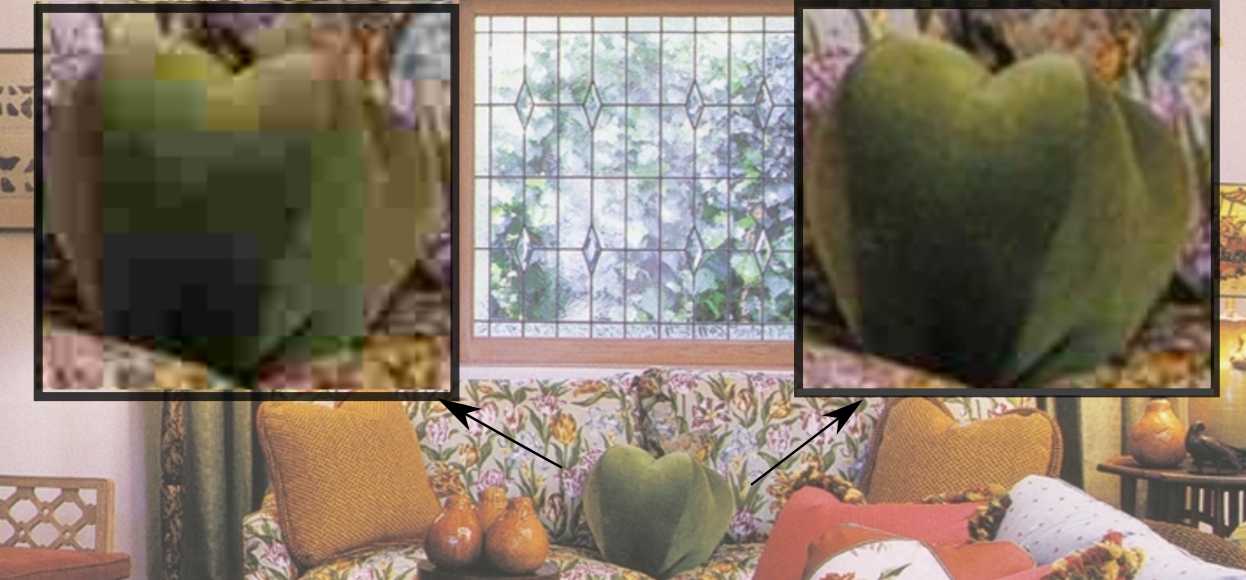
\includegraphics[scale=0.34]{figures/semantic/arrow_small.png}
    \caption[Comparison with JPEG]{Comparison of compression of semantic objects in standard \textsc{jpeg}[left] and our model [right]\label{fig_compressing_demo}}
\end{figure}

\textsc{cnn}s have been successfully applied to a variety of computer vision tasks \cite{krizhevsky2012imagenet}.
The feature extraction and transfer learning capabilities of \textsc{cnn}s are well known \cite{zeiler2014visualizing}, as are their ability to classify images by their most prominent object \cite{he2015deep}, and compute a bounding box \cite{girshick2014rich}.
Some success has been obtained in predicting the visual saliency map of a given image \cite{jiang2015salicon},\cite{kummerer2014deep}.
Previous work has shown that semantic object detection has a variety of advantages over saliency maps \cite{mnih2014recurrent}, \cite{zund2013content}.
Semantic detection recognizes discrete objects and is thus able to generate maps that are more coherent for human perception.
Visual saliency models are based on human eye fixations, and thus produce results which do not capture object boundaries \cite{kummerer2014deep}.
This is evident in the results obtained by Stella et al \cite{stella2009image}, in which image compression is guided by a multi-scale saliency map, and the obtained images show blurred edges and soft focus.

We present a \textsc{cnn} designed to locate multiple regions of interest (\textsc{roi}) within a single image.
Our model differs from traditional object detection models like \cite{dai2016r}, \cite{girshick2014rich} as these models are restricted to detecting a single salient object in an image.
It captures the structure of the depicted scene and thus maintains the integrity of semantic objects, unlike results produced using human eye fixations \cite{liu2015predicting}.
We produce a single class-invariant feature map by learning separate feature maps for each of a set of object classes and then summing over the top features.
Because this task does not require precise identification of object boundaries, our system is able to capture multiple salient regions of an image in a single pass, as opposed to standard object detection \textsc{cnn}s, which require multiple passes over the image to identify and locate multiple objects.
Model training need only be done offline, and encoding with our model employs a standard \textsc{jpeg} encoder combined with efficient computation of saliency maps (over 60 images per second for 1920x1080 using a Titan X Maxwell \textsc{gpu}).
A key advantage of our approach is that its compressed output can be decoded by any standard off-the-shelf \textsc{jpeg} implementation.  It serves to maintain the existing decoding complexity, the primary issue for distribution of electronic media.
% done: Move this citation to past work, make it not be negative -- decided against adding this line
%In contrast to grid based features as described by Yuri et al \cite{reznik2013coding} our features are scale and translation invariant, which allows application of the model to a wider class of images.


% TODO fix section numbers
Section 2 reviews \textsc{cnn} techniques used for object localization, semantic segmentation and class activation maps. We also discuss merits of using our technique over these methods.
Section 3 presents our new model which can generate a map showing multiple regions of interest. In Section 4 show how we combine this map to make \textsc{jpeg} semantically aware.
Sections 5 presents experimental results on a variety of image datasets and metrics. Section 6 concludes with future areas for research.

%%%%%%%%%%%%%%%%%%%%%%%%%%%%%%%%%%%%%%%%%%%%%%%%%%%%%%%%%%%%%%%%%%%%%%%%%%%%%%%%%%%%%%%%%%%%%%%%%%%%%%%%%%%%%%%%%%%%%%%%%%%%%%%%%%%%%%

\section{Review of localization using CNNs}
%%%%%%%%%%%%%%%%%%%%%%%%%%%%%%%%%%%%%%%%%%%%%%%%%%%%%%%%%%%%%%%%%%%%%%%%%%%%%%%%%

\textsc{cnn}s are multi-layered feed-forward architectures where the learned features at each level are the weights of the convolution filters to be applied to the output of the previous level. Learning is done via gradient-based optimization \cite{lecun1995convolutional}.
\textsc{cnn}s differ from fully connected neural networks in that the dimensions of the learned convolution filters are, in general, much smaller than the dimensions of the input image, so the learned features are forced to be localized in space. Also, the convolution operation uses the same weight kernel at every image location, so feature detection is spatially invariant.


Given an image $x$, and a convolution filter of size $n \times n$, then a convolutional layer performs the operation shown in equation \ref{eqn_cnn}, where $\mathbf{W}$ is the learned filter.

\begin{equation}
    y_{ij} = \sum_{a=0}^{n} \sum_{b=0}^{n} \; \mathbf{W}_{ab} \; x_{(i+a)(j+b)}
    \label{eqn_cnn}
\end{equation}

In practice, multiple filters are learned in parallel within each layer, and thus the output of a convolution layer is a 3-\textit{d} feature map, where the depth represents the number of filters. The number of features in a given layer is a design choice, and may differ from layer to layer.
\textsc{cnn}s include a max pooling \cite{lecun1995convolutional} step after every or every other layer of convolution, in which the height and width of the feature map (filter response) are reduced by replacing several neighboring activations (coefficients), generally within a square window, with a single activation equal to the maximum within that window.  This pooling operation is strided, but the size of the pooling window can be greater than the stride, so windows can overlap.
This results in down-sampling of input data, and filters applied to such a map will have a larger receptive field (spatial support in the pixel space) for a given kernel size, thus reducing the number of parameters of the \textsc{cnn} model and allowing the training of much deeper networks.
%Max pooling performed with a stride of $ k \times k $ will reduce a feature matrix of size $ N \times N $ to $ \frac{N}{k} \times \frac{N}{k}$.
This does not change the depth of the feature map, but only its width and height.
In practice, pooling windows are typically of size $2 \times 2$ or $4 \times 4$, with a stride of two, which reduces the number activations by 75\%.
\textsc{cnn}s apply some form of non-linear operation such as sigmoid $ (1-e^{-x})^{-1} $ or linear rectifier $max(0,x)$ on the output of each convolution operation.


Region-based \textsc{cnn}s use a moving window to maximize the posterior of the presence of an object \cite{girshick2015fast}.
%However, this is computationally expensive as it requires looking for all possible classes in all possible regions.
Faster \textsc{rcnn}s \cite{ren2015faster} have been proposed, but they are still computationally expensive and are limited to determining the presence or absence of a single class of object within the entire image.
%Moving-window methods are also limited in their ability to provide tight bounds on the location of an object.
Moving-window methods are able to produce rectangular bounding boxes, but cannot produce object silhouettes.
In contrast, recent deep learning models proposed for semantic segmentation \cite{long2015fully}, \cite{girshick2014rich}, \cite{zheng2015conditional} are very good at drawing a close border around the objects.
However, these methods do not scale well to more than a small number of object categories (e.g. $20$) \cite{everingham2010pascal}.
Segmentation methods typically seek to produce a hard boundary for the object, in which every pixel is labeled as either part of the object or part of the background.
In contrast, class activation mapping produces a fuzzy boundary and is therefore able to capture pixels which are not part of any particular object, but are still salient to some spatial interaction between objects.
Segmentation techniques are also currently limited by the requirement for strongly-labeled data for training.
Obtaining training data where the locations of all the objects in the images are tagged is expensive and not scalable \cite{everingham2010pascal}. Our approach only requires image-level labels of object classes, without pixel-level annotation or bounding-box localization.

%\section{Class Activation Mapping}
%%%%%%%%%%%%%%%%%%%%%%%%%%%%%%%%%%%%%%%%
%Convolution filters learned from natural images are sensitive to the object classes in the training data \cite{oquab2015object}, \cite{lin2013network}.
%In other words, regions of an image which contain relevant objects tend to produce high activations when convolved with learned filters, while regions that do not contain any object class have lower activations, and this is particularly true for the deeper levels of the \textsc{cnn}.
In a traditional \textsc{cnn}, there are two fully-connected (non-convolutional) layers as the final layers of the network. 
%neurons at end of the pipeline, with connections to every activation from the feature map of the previous layer.
The final layer has one neuron for every class in the training data, and the final step in the inference is to normalize the activations of the last layer to sum to one.
The second to last layer, however, is fully connected to the last convolution layer, and a non-linearity is applied to its activations.
The authors of \cite{oquab2015object}, \cite{zhou2015learning} modify this second to last layer to allow for class localization.
In their architecture, the second to last layer is not learned, but consists of one neuron for each feature map, which has fixed  equally-weighted connections to each activation of its corresponding map.
%They suggest one neuron for each feature map from the last convolution layer, and this neuron has connections of equal weight to every activation of its feature map and no connections to any other feature map.
No non-linearity is applied to the outputs of these neurons, so that each activation in this layer represents the global spatial average of one feature map from the previous layer.
Since the output of this layer is connected directly to the classification layer, each class will in essence learn a weight for each feature map from the final convolution layer.
Thus, given an image and a class, the classification weights for that class can be used to re-weight the layers of activations of the final convolution layer on that image.
These activations can be collapsed along the feature axis to create a class activation map, spatially localizing the best evidence for that class within that image. 
% done discuss the definition
%Taking the spatial average of the feature map (global average pooling) at the last convolution layer reveals possible locations of objects within the image \cite{oquab2015object}, \cite{zhou2015learning}. 
This is used to make Class Activation Maps (CAM), which shows the probability distribution of the most likely class.

While standard max pooling combines spatially local activations for each feature independently, `global max pooling' instead combines the activations of all features for each spatial location.  
%This collapses the feature map to two spatial dimensions by reducing the $D$ features at each location to a single maximum value.
If the activation of a convolution layer is of size $ M \times N \times D $ where $M$ and $N$ are the spatial dimensions of feature activations and $D$ denotes the number of features in the feature map, then after `global max pooling', the size of activations becomes $M \times N$.
It is important to note that global average pooling is performed in lieu of a final fully-connected layer (or perceptron), which is often used in image classification tasks \cite{Simonyan2014VeryDC}.
Fully-connected layers have dense connections across all neurons and thus do not preserve spatial locality of activations.
The substitution of a global max pooling layer retains this locality property in exchange for a fractional loss of classification accuracy\cite{oquab2015object}.
Pooling of feature maps is probabilistic \cite{li2015beyond}, which means the most salient object is not always the one with highest activation across the feature map. 
If we plot the activation of each feature on the $2$-dimensional map and overlay them on each other, we find significant overlap of regions of high activations.
This means taking a `global max pooling' would lead to missing some. 
Zhou \cite{zhou2015learning} reported that they obtained better localization by performing `global average pooling' instead of `global max pooling'. 
This is because taking an average across the feature map ensures each detected object has consistently high activations across many features, instead of a single maximal activation of one feature.
%The application of GAP after the final layer of convolution $ y_{ij} $ over $\mathbf{D}$ features would result in --
%CAM is obtained by taking output of the last convolution layer $f(x,y)$, and taking a weighted sum across the feature map.
% todo: what class is the CAM in the figure for?
Figure~\ref{fig_comparison_of_map} (c) shows an example of such a map, the equation of which is given by
%the CAM for the class girl overlayed on the original image, where each pixel value is given by

\begin{equation}
    M_c(x,y) = \sum_{d \; \epsilon \; \mathbf{D}} w^{c}_{d} \; f_d(x,y)
    \label{eqn_gap}
\end{equation}

{\setlength{\parindent}{0cm} where $ w^{c}_{d} $ is the learned weight of class $c$ for feature map $d$.
%in the supervised training, and $\mathbf{D}$ the set of the numbers of filters for each layer.
% M is referred to as class activation mapping (CAM) ~\ref{fig_comparison_of_map}.
% It is used to generate discriminative localization for the most probable class.
Training for \textsc{cam} minimizes the cross entropy between objects' true probability distribution over classes (all mass given to the true class) and the predicted distribution, which is obtained as }

\begin{equation}
    P(c) = \frac{\text{exp}(\sum_{xy}{M_c(x,y)})}{\sum_c \text{exp}(\sum_{xy}{M_c(x,y)})}
    \label{eqn_posterior}
\end{equation}

Since \textsc{cam}s are trained to maximize posterior probability for the class, they tend to only highlight a single most prominent object.
This makes them useful for studying the output of \textsc{cnn}s, but not well suited to more general semantic saliency, as real world images  typically contain multiple objects of interest.
This has practical applications in understanding and visualizing convolution neural networks but is less applicable to real world images, which typically contain multiple objects of interest.
Without using standard resolution, color-space or types of object classes it is hard to use such systems to extract semantic information from the images.

\section{Multi-Structure Region of Interest}
%%%%%%%%%%%%%%%%%%%%%%%%%%%%%%%%%%%%%%%%%%%%%%%%%%%%%%%%%%%%%%%%%%%%%%%%%%%%%%%%
We have developed a variant of \textsc{cam} which balances the activation for multiple objects and thus does not suffer from the issues of global average pooling.
Our method, \textit{Multi-Structure Region of Interest} (MS-ROI), allows us to effectively train on localization tasks independent of the number of classes.
For the purposes of semantic compression, obtaining a tight bound on the objects is not important. However, identifying and approximately locating all the objects is critical.
We propose a set of 3D feature maps in which each feature map is learned for an individual class, and is learned independently of the maps for other classes.
For $ \mathbf{L} $ layers, where each layer $l$ contains $d_l$ features, an image of size $ n \times n $, and with $\mathbf{C}$ classes, this results in a total activation size of

\begin{equation*}
    \sum_{l \; \epsilon \; \mathbf{L}}{d_l \times \mathbf{C} \times \frac{n}{k^l} \times \frac{n}{k^l}}
\end{equation*}

where $k$ is the max pooling stride size.
This is computationally very expensive, and not practical for real world data.
\textsc{cnn}s designed for full-scale color images have many filters per layer and are several layers deep.
For such networks, learning a model with that many parameters would be unfeasible in terms of computational requirements.
We propose two techniques to make this idea feasible for large networks: 
% (i) reduce the number of classes and increase the inter-class variance by combining similar classes, and  
% (ii) share feature maps across classes to jointly learn lower level features.

\begin{enumerate}[i]
	 \item Reduce the number of classes and increase the inter-class variance by combining similar classes
    \item Share feature maps across classes to jointly learn lower level features
\end{enumerate}

Most \textsc{cnn} models are built for classification on the Large Scale Visual Recognition Challenge, commonly known as ImageNet.
\footnote{http://image-net.org/challenges/LSVRC/}.
ImageNet has one thousand classes and many of the classes are fine-grained delineations of various types of animals, flowers and other objects.
We significantly reduce the number of classes by collapsing these sets of similar classes to a single, more general class.
This is desirable because, for the purpose of selecting a class invariant `region of interest,' we do not care about the differences between Siberian husky and Eskimo dog or between Lace-flower and Tuberose.
As long as objects of these combined classes have similar structure and are within the same general category, the map produced will be almost identical.
Details of the combined classes used in our model are provided in the Experimental Results section.

It is self-evident that most images contain only a few classes and thus it is computationally inefficient to build a separate feature map for every class.
More importantly, many classes have similar lower-level features, even when the number of classes is relatively small.
The first few layers of a \textsc{cnn} learn filters which recognize small edges and motifs \cite{zeiler2014visualizing}, which are found across a wide variety of object classes.
Therefore, we propose parameter sharing across the feature maps for different classes.
This reduces the number of parameters and also allows for the joint learning of these shared, low-level features.

\begin{figure}[H]
    \centering
    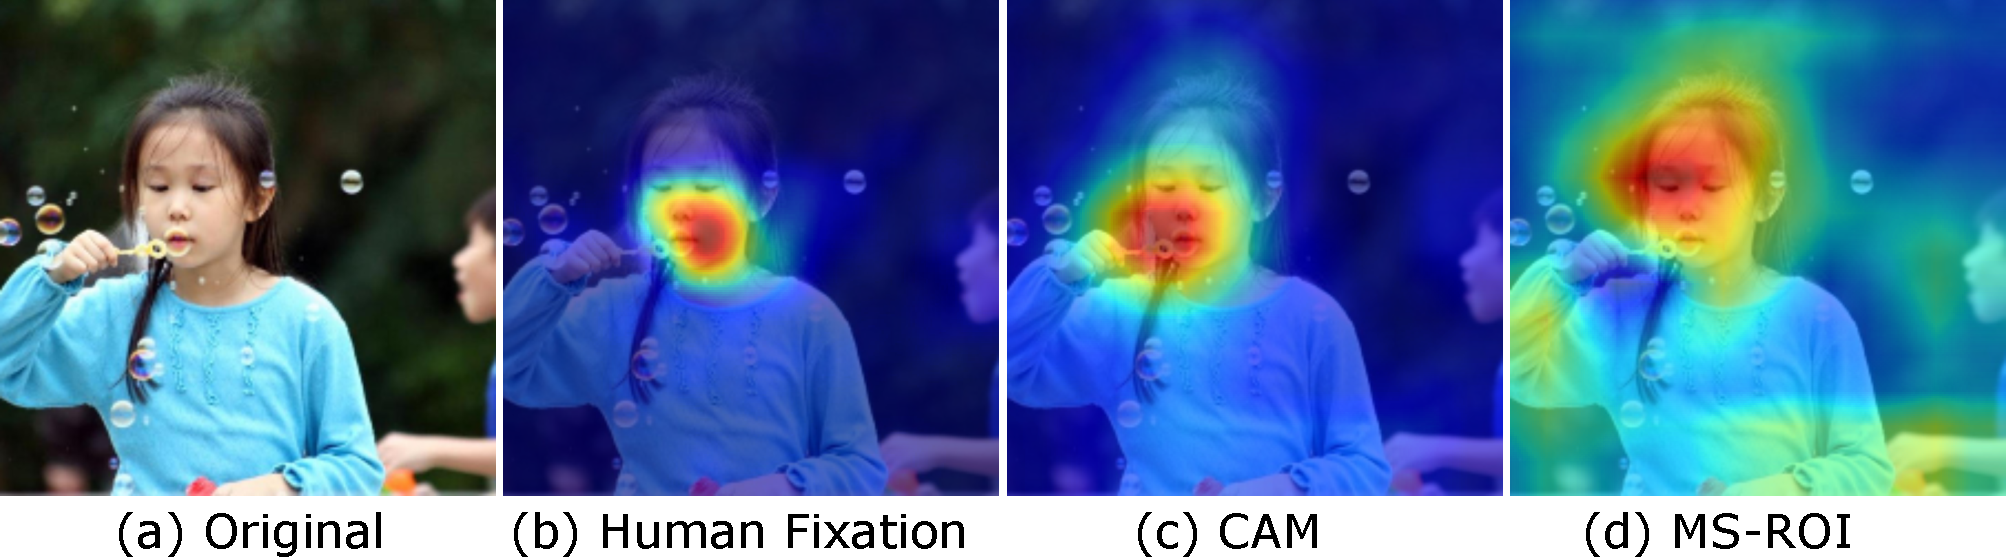
\includegraphics[scale=0.45]{figures/semantic/girl_compression.pdf}
    \caption[MSROI vs CAM vs Saliency]{Comparison of various methods of detecting objects in an image \label{fig_comparison_of_map}}
\end{figure}

Although we do not restrict ourselves to a single most-probable class, it is desirable to eliminate the effects of activations for classes which are not present in the image.  
In order to accomplish this, we propose a thresholding operation which discards those classes whose learned features do not have a sufficiently large total activation when summed across all features and across the entire image.  
Let $Z^c_l$ denote the total sum of the activations of layer $\ell$ for all feature maps for a given class $c$.
Since our feature map is a $4$-dimensional tensor, $Z^c_l$ can be obtained by summation of this tensor over the three non-class dimensions.

\begin{equation}
    Z^c_l = \sum_{d \; \epsilon \; \mathbf{D}} \sum_{x,y} f_d^c(x,y)
    \label{eqn_Zscore}
\end{equation}

Next, we use $Z^c_l$ to filter the classes. Computation of the multi-structure region of interest is shown below.

\begin{equation}
    \hat{M}(x,y) = \sum_{c \; \epsilon \; \mathbf{c} }
    \begin{cases}
        \sum_d f_d^c(x,y), & \text{if}\ Z^c_l > T \\
        \phantom{this_is_empty} \\
      0 & \text{otherwise}
    \end{cases}
    \label{eqn_msroi}
\end{equation}

We use the symbol $\hat{M}$ to denote the multi-structure map generated by our proposed model in order to contrast it with the map generated using standard \textsc{cam} models, $ M $.
$ \hat{M} $ is a sum over all classes with total activations $Z^c_l$ beyond a threshold value $T$.
$T$ is determined during the training or chosen as a hyper-parameter for learning. 
In practice, it is sufficient to \textit{argsort} $Z^c_l$ and pick the top five classes and combine them via a sum weighted by their rank. 
It should be noted that, because $ \hat{M} $ is no longer a reflection of the class of the image, we use the term `region of interest'.

A comparison of our model (MS-ROI) with \textsc{cam} and human fixation is shown in Figure~\ref{fig_comparison_of_map}. 
Only our model identifies the face of the boy on the right as well the hands of both children at the bottom. 
When doing compression, it is important that we do not lower the quality of body extremities or other objects which other models may not identify as critical to the primary object class of the image.
If a human annotator were to paint the areas which should be compressed at better quality, we believe the annotated area would be closer to that captured by our model.

To train the model to maximize the detection of all objects, instead of using a softmax function as in equation \ref{eqn_posterior}, we use sigmoid, which does not marginalize the posterior over the classes.
Thus the likelihood of a class $c$ is given by equation~\ref{eqn_our_posterior}. 

\begin{equation}
    P(c) = \frac{1}{1 + \text{exp}(Z^c_l)}
    \label{eqn_our_posterior}
\end{equation}

\section{Integrating MS-ROI map with JPEG}
%%%%%%%%%%%%%%%%%%%%%%%%%%%%%%%%%%%%%%%%%%%%%%%%%%%%%%%%%%%%%%%%%%%%%%%%%%%%%%%%
We obtain from MS-ROI a saliency value for each pixel in the range [0,1], where 1 indicates maximum saliency.
Then discretize these saliency values into $k$ levels, where $k$ is a tune-able hyper-parameter.
The lowest level contains pixels of saliency $[0,1/k]$, the second level contains pixels of saliency $(1/k,2/k]$ and so forth.
We next select a range of \textsc{jpeg} quality levels, $Q_l$ to $Q_h$.  Each saliency level will be compressed using a $Q$ value drawn from this range, corresponding to that level.
In other words, saliency level $n$, with saliency range $[n/k,(n+1)/k]$ will be compressed using 

\begin{equation}
Q_n = Q_l + \frac{n*(Q_h - Q_l)}{k}
\end{equation}


For each level $l \le n \le h$, we obtain a decoded \textsc{jpeg} of the image after encoding at quality level $Q_n$.
For each $8 \times 8$ block of our output image, we select the block of color values obtained by the \textsc{jpeg} corresponding to that block's saliency level.  This mosiac of blocks is finally compressed using a standard \textsc{jpeg} encoder with the desired output quality to produce a file which can be decoded by any off-the-shelf \textsc{jpeg} decoder.

Details of our choices for $k$, $Q_l$ and $Q_h$, as well as target image sizes are provided in the next section.  A wider range of $Q_l$ and $Q_h$ will tend to produce stronger results, but at the expense of very poor quality in non-salient regions.

\begin{algorithm}[H]
\SetKwInOut{Input}{Input}
\SetKwInOut{Output}{Output}

    \Input{Image: I}
    \Output{Image: O, same dimensions as I}
    Let $Q_{l \cdot h}$ be N fixed values in range l to h
    
    \For{b $\gets 8 \times 8$ blocks in I}{
        $Q_i = \hat{M}$[b] \#Nearest\ quantized\ level
        
        I'[b] $\gets$ JPEG \{I[b], $Q_i$\}
    }
    O $\gets$ JPEG\{I', $Q_f$\}
\caption[Encoding with MSROI]{JPEG Encoding with MSROI}
\label{alg:encoding}
\end{algorithm}

Encoding of image using MSROI on a JPEG standard can be summarized as shown by algorithm ~\ref{alg:encoding}.

Figure ~\ref{fig_encoding_steps} shows the steps of taking an image and using the MSROI map to obtain the final encoded image.

\begin{figure}[H]
    \centering
    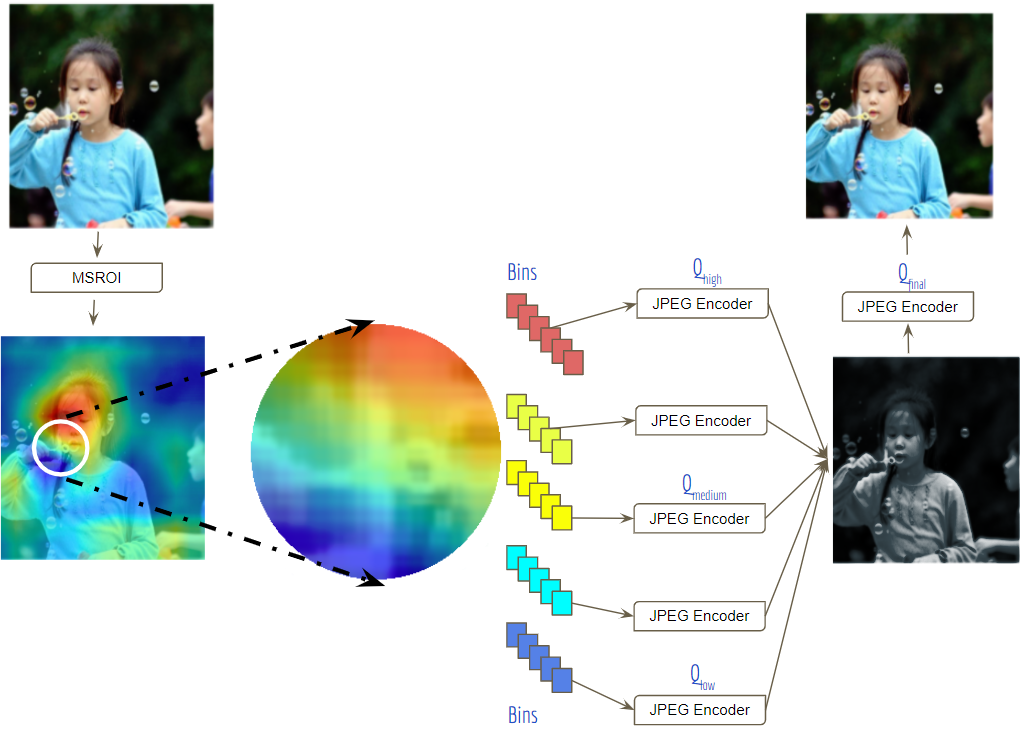
\includegraphics[scale=0.45]{figures/semantic/variable_q_jpeg.png}
    \caption[Encoding with MSROI]{Process of combining MSROI maps to obtain final encoded image \label{fig_encoding_steps}}
\end{figure}


\section{Experimental Results}
%%%%%%%%%%%%%%%%%%%%%%%%%%%%%%%%%%%%%%%%%%%%%%%%%%%%%%%%%%%%%%%%%%%%%%%%%%%%%%%%%
We trained our model with the Caltech-256 dataset \cite{griffin2007caltech}, which contains 256 classes of man-made and natural objects, common plants and animals, buildings, etc.

We believe this offers a good balance between covering more classes as compared to CIFAR-100 which contains only 100 classes, and avoiding overly finely-grained classes as in ImageNet with 1000 classes \cite{imagenet_cvpr09}.
For the results reported here, we experimented with several stacked layers of convolution as shown in the diagram below:
\begin{equation*}
    \text{IMAGE} \longmapsto \bigg[ \big[ \text{CONV} \rightarrow \text{RELU}\big]^2 \rightarrow \text{MAXPOOL} \bigg]^5 \longmapsto \text{MS-ROI} \longmapsto \text{MAP}
\end{equation*}


$\text{MS-ROI}$ refers to the operation shown in the equation~\ref{eqn_msroi}.
To obtain the final image we discretize the heat-map into five levels and use \textsc{jpeg} quality levels $Q$ in increments of ten from $Q_l=30$ to $Q_h=70$.
For all experiments, the file size of the standard \textsc{jpeg} image and the \textsc{jpeg} obtained from our model were kept within $\pm1\%$ of each other.
On average, salient regions were compressed at $Q_f=65$, and non-salient regions were compressed at $Q=45$.
The average $Q$ for the final image generated using our model was $55$, whereas for all standard \textsc{jpeg} samples, $Q$ was chosen to be 50. It should be noted that even though images are at different $Q$ they have same size.

\begin{figure}[H]
    \centering
    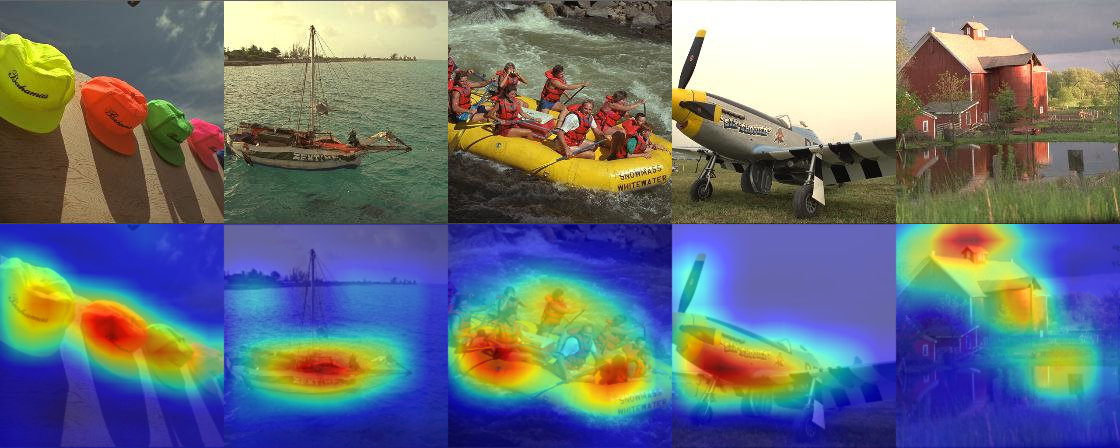
\includegraphics[scale=0.37]{figures/semantic/all_images_small.png}
    \caption[Results on KODAK]{Sample of our map for five KODAK images.\label{fig_kodak_combo}}
\end{figure}

We tested on the Kodak PhotoCD set (24 images) and the the MIT dataset (2,000 images).
Kodak is a well known dataset consisting primarily of natural outdoor color images.
Figure~\ref{fig_kodak_combo} shows a sample of five of these images, along with the corresponding heatmaps generated by our algorithm; the first four show typical results which strongly capture the salient content of the images, while the fifth is a rare case of partial failure, in which the heatmap does not fully capture all salient regions.
The MIT set allows us to compare results across twenty categories. In Table~\ref{tbl_results} we only report averaged results across `Outdoor Man-made' and `Outdoor Natural' categories (200 images), as these categories are likely to contain multiple semantic objects, and are therefore appropriate for our method.
Both datasets contain images of smaller resolutions, but the effectiveness of perceptual compression is more pronounced for larger images.
Therefore, we additionally selected a very large image of resolution $8705\times8400$, which we scale to a range of sizes to demonstrate the effectiveness of our system at a variety of resolutions.
See Figure~\ref{fig_size} for the image sizes used in this experiment.
Both Figure~\ref{fig_size} and Figure~\ref{fig_mit} show the \texttt{PSNR-HVS} difference between our model and standard \textsc{jpeg}. Positive values indicate our model has higher performance compared to standard \textsc{jpeg}.
In addition to an array of standard quality metrics, we also report a \texttt{PSNR} value calculated only for those regions our method has identified as salient, which we term \texttt{PSNR-S}.
By examining only regions of high semantic saliency, this metric demonstrates that our compression method is indeed able to preserve visual quality in targeted regions, without sacrificing performance on traditional image-level quality metrics or compression ratio.
It should be noted that the validity of this metric is dependent on the correctness of the underlying saliency map, and thus should only be interpreted to demonstrate the success of the final image construction in preserving details highlighted by that map.

\begin{table}[H]
% \footnotesize
\centering
\rowcolors{1}{White}{Gray}
\begin{tabular}{lccccccc}
			 \toprule
               & \texttt{PSNR-S} \phantom{so} & \texttt{PSNR} \phantom{so} & \texttt{PSNR-HVS} \phantom{so}& \texttt{PSNR-HVSM} \phantom{so}& \texttt{SSIM} \phantom{so}& \texttt{MS-SSIM} \phantom{so}& \texttt{VIFP}\phantom{so} \\
              \midrule
              & \multicolumn{6}{c}{Kodak PhotoCD [24 images]}   &                        \\
              \midrule
Std \textsc{jpeg} &   33.91   & 34.70     & 34.92          & 42.19  & 0.969  & 0.991 & 0.626      \\
% 			  \midrule
			  \cline{2-8}
Our model &  39.16    & 34.82    & 35.05          & 42.33  & 0.969  & 0.991 Carlini2017TowardsET& 0.629     \\
			  \midrule
              & \multicolumn{6}{c}{MIT Saliency Benchmark [Outdoor Man-made + Natural, 200 images]} &              \\
			  \midrule
Std \textsc{jpeg} & 36.9 & 31.84    & 35.91   & 45.37 & 0.893 & 0.982     & 0.521      \\
% 			  \midrule
			  \cline{2-8}
Our model & 40.8 & 32.16   & 36.32   & 45.62 &  0.917 & 0.990      & 0.529      \\
			  \midrule
              & \multicolumn{6}{c}{Re-sized images of a very large image, see fig:~\ref{fig_size} [20 images]} &          \\
			  \midrule
Std \textsc{jpeg} & 35.4   & 27.46  & 33.12 & 43.26     & 0.912 & 0.988 & 0.494     \\
% 			  \midrule
			  \cline{2-8}
Our model & 39.6  & 28.67  & 34.63 & 44.89     & 0.915 & 0.991 & 0.522     \\
			  \toprule
\end{tabular}
\caption[Results across various datasets]{Results across datasets \label{tbl_results}}
\end{table}
        
\begin{figure}[H]
    \centering
    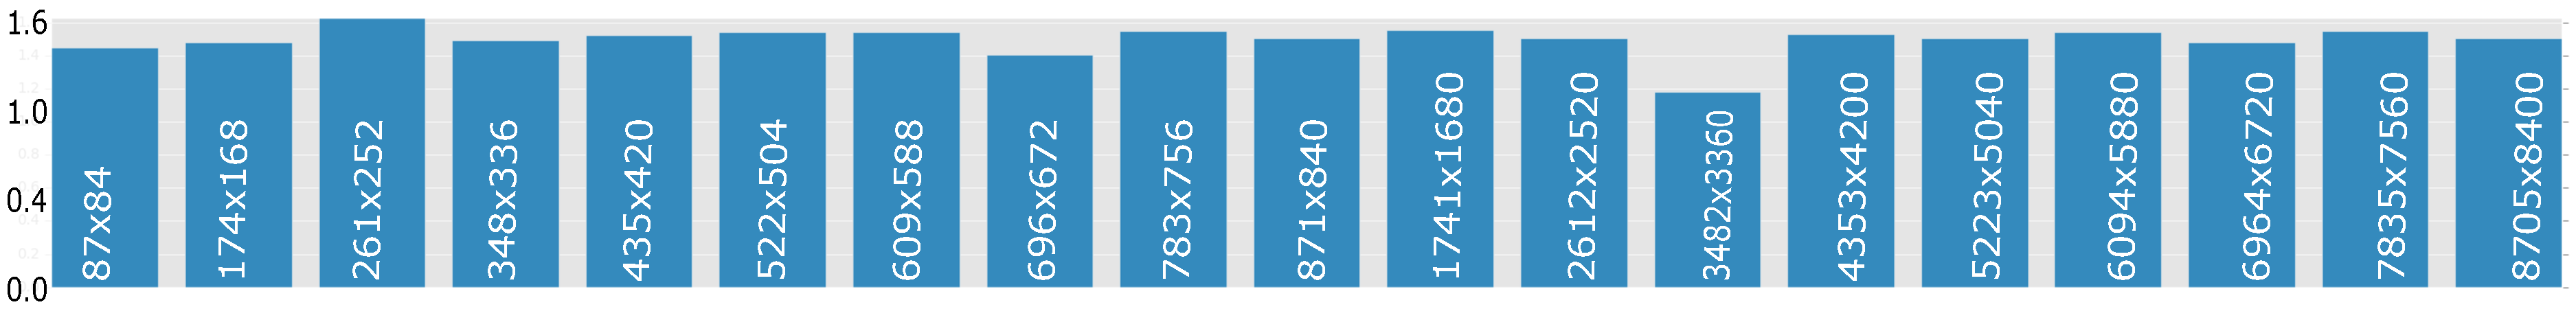
\includegraphics[scale=0.23]{figures/semantic/image_size.pdf}
    \caption[Impact on Image Size]{\texttt{PSNR-HVS} of our model - \textsc{jpeg} across various image size (higher is better). \label{fig_size}}
\end{figure}

\begin{figure}[H]
    \centering
    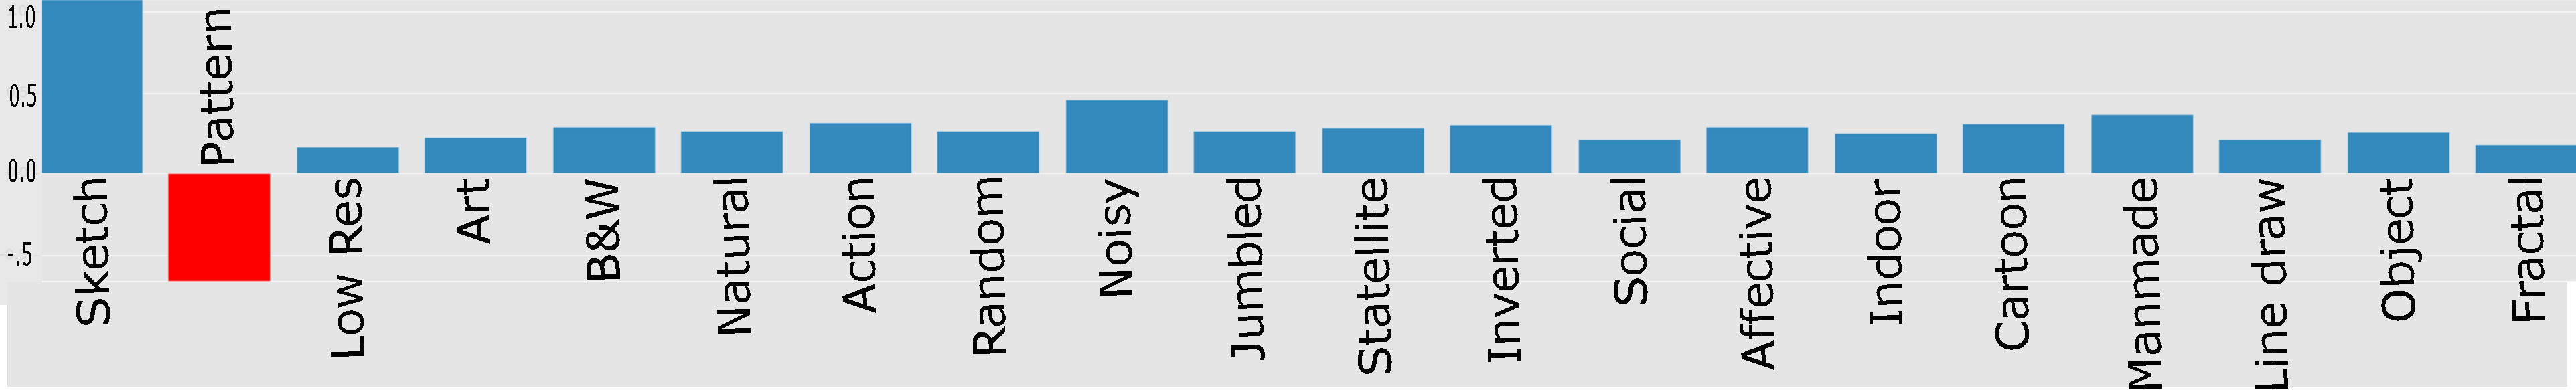
\includegraphics[scale=0.23]{figures/semantic/image_mit.pdf}
    \caption[Impact on Image Type]{\texttt{PSNR-HVS} of our model - \textsc{jpeg} across various categories of MIT Saliency dataset (higher is better). \label{fig_mit}}
\end{figure}

\section{Discussion}
%%%%%%%%%%%%%%%%%%%%%%%%%%%%%%%%%%%%%%%%%%%%%%%%%%%%%%%%%%%%%%%%%%%%%%%%%%%%%%%%
While the comparison of metrics in Table~\ref{tbl_results} on standard \textsc{jpeg} and variable quality \textsc{jpeg} using our  generated map is similar, it should be noted that these metrics still lack ability to judge human perception. 
It is evident from the results that the salient objects have significantly higher \texttt{PSNR-S}, yet maintains overall \texttt{PSNR} and the file size.
We believe we have effectively created a model to make \textsc{jpeg} semantically aware without sacrificing overall image quality.
% done  fix "better" -- no need, commented that section
We know from the \textsc{jpeg} standard that images compressed with higher $Q$ better, and by design our model compresses the salient objects with higher $Q$; see Figure~\ref{fig_compressing_demo} for qualitative evaluation.

The results in Table~\ref{tbl_results} show the success of our method in maintaining or improving performance on traditional image quality metrics.
Further, given the efficacy of our method in identifying multiple regions of interest, the \texttt{PSNR-S} measurements demonstrate the power of our method to produce superior visual quality in subjectively important regions.

When we look at Figure~\ref{fig_compressing_demo} we see the difference in quality of the salient object.  
Our model consistently outperforms standard \textsc{jpeg} on \texttt{SSIM} and \texttt{MS-SSIM} metric.
These metrics measure the inherent structures in the image and Richter et al \cite{richter2009ms} \cite{richter2011ssim} has shown efficacy of these metric for image compression.

Figure~\ref{fig_mit} shows the performance of our model across all categories of the MIT dataset.
Performance was strongest in categories like `Outdoor Natural', `Outdoor Man Made', `Action' and `Object', while categories like `Line Drawing', `Fractal' and `Low Resolution' showed the least improvement.
Not surprisingly, the category `Pattern', which lacks semantic objects, is the only category where our model did not improve upon standard \textsc{jpeg}.
Figure~\ref{fig_size} shows results on the same image scaled to different sizes. 
Because our model benefits from the scale-invariance of \textsc{cnn}s, we are able to preserve performance across a wide range of input sizes.
Performance of our model on \texttt{PSNR-HVS} is consistent across all tested sizes. \textsc{cnn}s are able to learn scale-invariant features, and therefore the same object at any size should always be classified similarly.
Our model preserves this feature even when looking for multiple objects.


    

%% Storer's version
\section{Conclusion}
We have presented a model which can learn to detect multiple objects at any scale and generate a map of multiple semantically salient image regions.
This provides sufficient information to perform variable-quality image compression, without providing a precise semantic segmentation.
Unlike region-based models, our model does not have to iterate over many windows.
We sacrifice exact localization for the ability to detect multiple salient objects.
%Using the output of our model as a map to perform variable-quality compression preserves the overall quality and size of the image, yet improves the visual quality of salient objects.
Our variable compression improves upon visual quality without sacrificing compression ratio. 
Encoding requires a single inference over the pre-trained model, the cost of which is reasonable when performed using a \textsc{gpu}, along with a standard \textsc{jpeg} encoder. The cost of decoding, which employs a standard, off-the-shelf \textsc{jpeg} decoder remains unchanged.
We believe it will be possible to incorporate our approach into other lossy compression methods such as \textsc{jpeg} 2000 and vector quantization, a subject of future work.
Improvements to the power of our underlying \textsc{cnn}, addressing evolving visual quality metrics, and other applications such as video compression, are also potential areas of future work.
